In this simulation, the same configuration for the neutron source as in the case of the TE material is used. The deposited energy in the  magnesium cylinder is:

\begin{figure}[!h]
\centering
\begin{minipage}{0.8\textwidth}
    \centering
    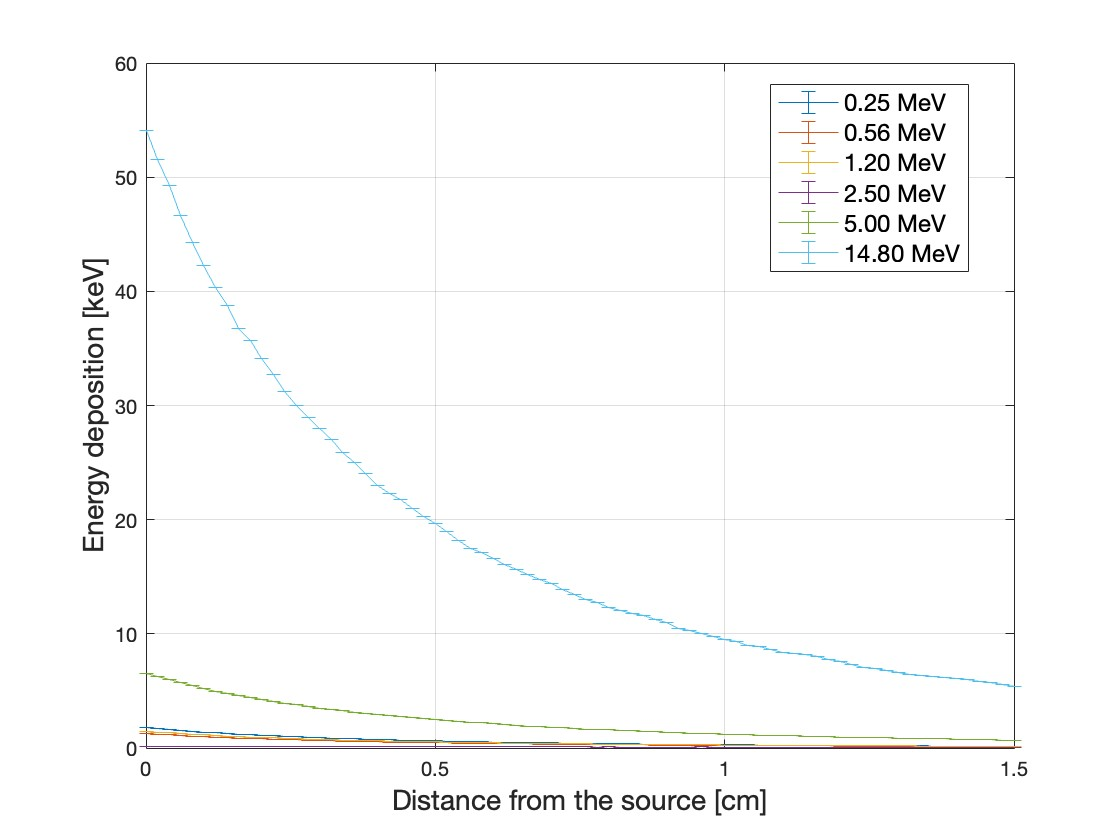
\includegraphics[width=\linewidth]{Master Thesis Manuel Galdon/figures/Build-up effect/Mg cylinder only.jpg}
    \label{fig:IC}
\end{minipage}
    \caption{Energy deposition plot of the magnesium cylinder plot using a plane neutron source at different energies. There is no gap between the source plane and the cylinder.}
    \label{fig:Mg cylinder with plane neutron source}
\end{figure}

According to the plot on Figure \ref{fig:Mg cylinder with plane neutron source}, there is apparently no build-up effect in this material. The difference between the energy deposition for the highest energy and the lower is too big to notice the response of the cylinder properly. For this reason, a close-up to the lowest energies is provided in the next plot: 
\newpage
\begin{figure}[!h]
\centering
\begin{minipage}{0.8\textwidth}
    %\renewcommand{\thefigure}{A} % Set the label of the first figure to A
    \centering
    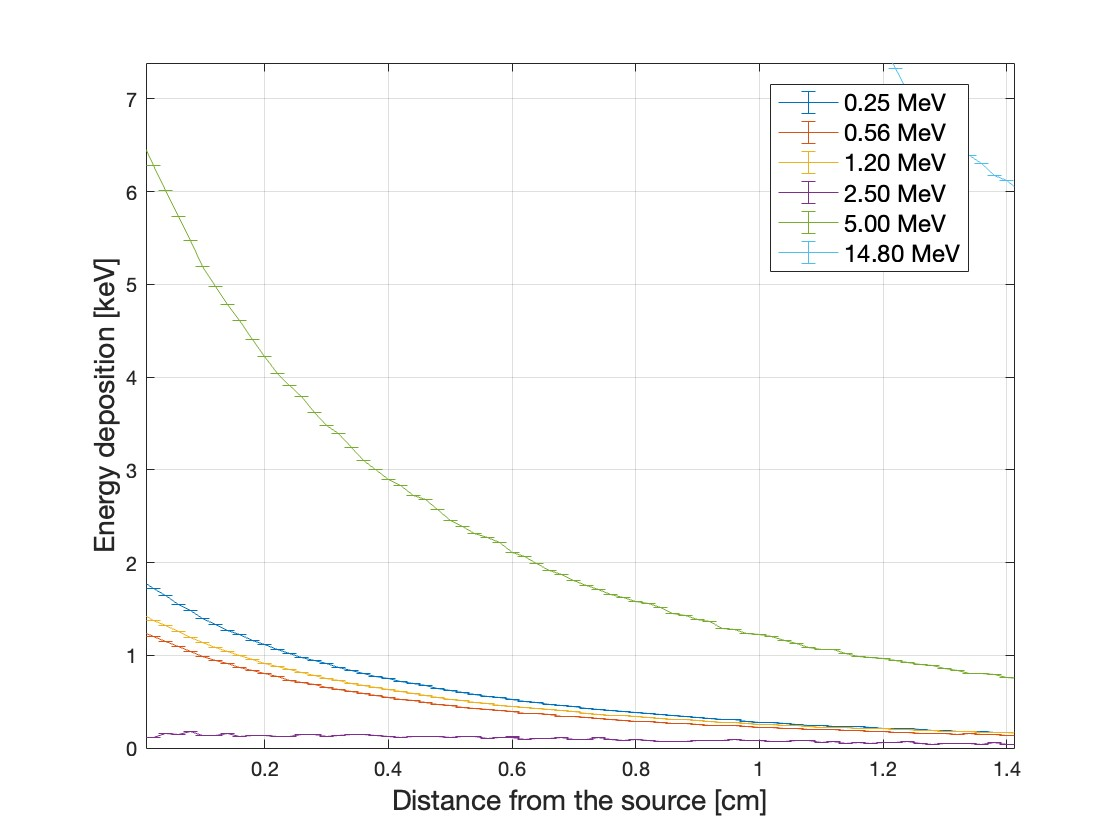
\includegraphics[width=\linewidth]{Master Thesis Manuel Galdon/figures/Build-up effect/Mg cylinder only - detail.jpg}
\end{minipage}
    \caption{Close-up of the energy deposition plot of the magnesium cylinder plot using a plane neutron source at different energies. There is no gap between the source plane and the cylinder.}
    \label{fig:Mg cylinder in detail with plane neutron source}
\end{figure}

The lines of the energies 0.25 and 2.5 \unit{\mega\electronvolt} appear to be switched, while the expected result should be a directly proportional relationship between the energy of the beam and the energy deposition.
This behaviour is due to the neutrons hitting the nuclei at a \textbf{resonance} energy for which the cross section of the atom grows significantly. In order to confirm that, the cross section of the magnesium against the energy of the incident neutron is plotted next:
\newpage
\begin{figure}[!h]
\centering
\begin{minipage}[t]{0.8\textwidth}
    \centering
    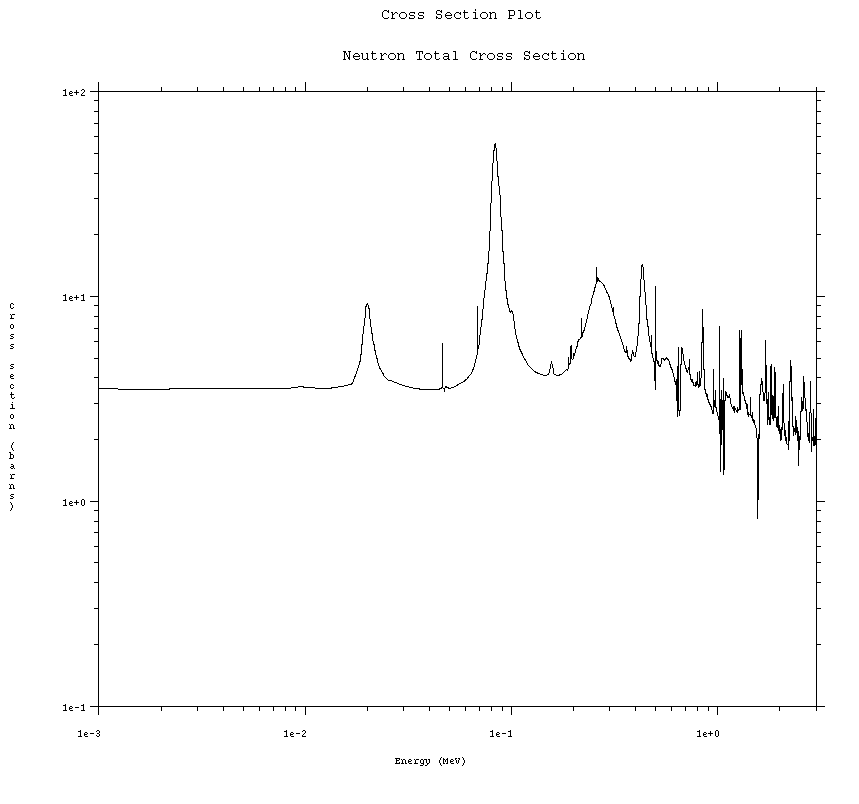
\includegraphics[width=\linewidth, height=9cm]{Master Thesis Manuel Galdon/figures/Build-up effect/cross section of Mg.png} 
    \caption{MCNP plot of the cross section in $barns$ of Mg.}
    \label{fig:Cross section of Mg}
\end{minipage}
\end{figure}

MCNP gives out the plots of the cross section of a material always in logarithmic scale. In this case, there is a sudden increase in the cross section for the energy of 0.25 \unit{\mega\electronvolt} and, for that value of the energy, the cross section is higher than for the case of 2.5 \unit{\mega\electronvolt}, which causes the plot in MCNP to show the energy deposition lines switched. 
